\documentclass[tikz]{standalone}

\usepackage{tkz-euclide}
\usetikzlibrary{calc, through}

\begin{document}
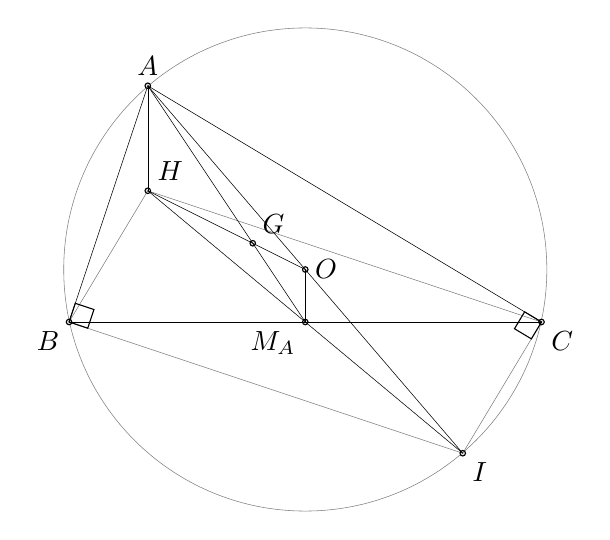
\begin{tikzpicture}
    % Define points
    \tkzDefPoints{0/3/A,-1/0/B,5/0/C}
    \tkzDefCircle[circum](A,B,C)
    \tkzGetPoint{O}
    \tkzGetLength{radius}

    \tkzDefMidPoint(B,C) \tkzGetPoint{M_A}
    \tkzDefMidPoint(C,A) \tkzGetPoint{M_B}

    % Define intersection
    \tkzInterLC(A,O)(O,A) \tkzGetSecondPoint{I}
    \tkzDefLine[orthogonal =through B](C,A) \tkzGetPoint{hb}
    \tkzDefLine[orthogonal =through C](A,B) \tkzGetPoint{hc}

    \tkzInterLL(B,hb)(C,A) \tkzGetPoint{H_B}
    \tkzInterLL(C,hc)(A,B) \tkzGetPoint{H_C}

    \tkzInterLL(B,H_B)(C,H_C) \tkzGetPoint{H}
    \tkzInterLL(A,M_A)(B,M_B) \tkzGetPoint{G}

    % Drawing
    \tkzDrawCircle(O,A)
    \tkzDrawPoints(H,M_A,G,I)
    \tkzDrawPoints(A,B,C,O)
    \tkzDrawSegments(A,B B,C C,A)
    \tkzDrawSegments(A,H A,M_A H,O A,I O,M_A)
    \tkzDrawSegments(H,I)
    \tkzDrawSegments[opacity=.5](B,H H,C C,I I,B)

    % Marking
    \tkzMarkRightAngle(A,B,I)
    \tkzMarkRightAngle(A,C,I)

    % Labeling
    \tkzLabelPoints[above](A)
    \tkzLabelPoints[right](O)
    \tkzLabelPoints[below left](B)
    \tkzLabelPoints[below right](C)
    \tkzLabelPoints[above right](H,G)
    \tkzLabelPoints[below left](M_A)
    \tkzLabelPoints[below right](I)

\end{tikzpicture}
\end{document}